% Compact PGFPlots panel for sampled qldpc_96_2_7_fixed_k_absorb_cap7 BSC correction-class derivative.
% Requires \usepackage{pgfplots} and \pgfplotsset{compat=1.18}.
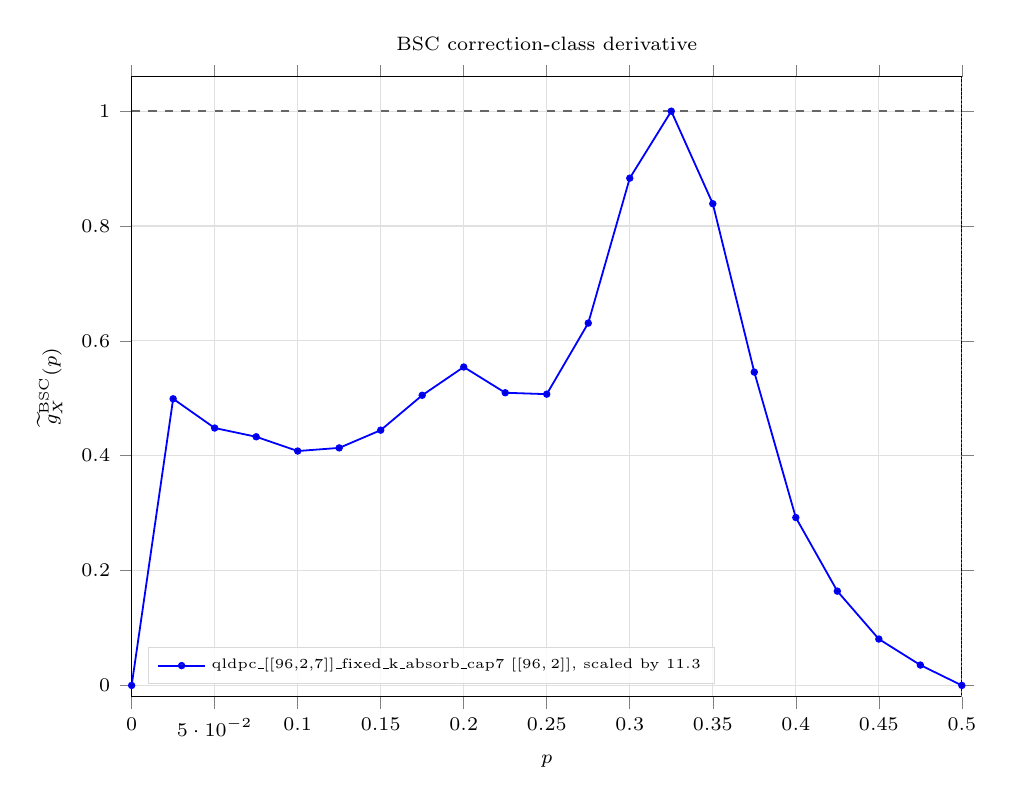
\begin{tikzpicture}
\begin{axis}[
  name=scaledBSCGEXITQldpc9627FixedKAbsorbCap7Axis,
  width=\linewidth,
  height=0.78\linewidth,
  title={BSC correction-class derivative},
  title style={font=\scriptsize},
  xlabel={$p$},
  ylabel={$\widetilde g_X^{\rm BSC}(p)$},
  xmin=0, xmax=0.5,
  ymin=-0.02, ymax=1.06,
  grid=both,
  major grid style={black!12},
  minor grid style={black!6},
  tick align=outside,
  tick label style={font=\scriptsize},
  label style={font=\scriptsize},
  legend cell align={left},
  legend style={draw=black!15, fill=white, fill opacity=0.82, text opacity=1, at={(0.02,0.02)}, anchor=south west, font=\tiny},
]
\addplot[black!60, densely dotted, line width=0.55pt, forget plot] coordinates {(0.5,-0.02) (0.5,1.06)};
\addplot[black!60, dashed, line width=0.55pt, forget plot] coordinates {(0,1) (0.5,1)};
\addplot+[color=blue, mark=*, mark size=1.0pt, line width=0.65pt]
coordinates {(0,0) (0.025,0.499137934742) (0.05,0.448262164534) (0.075,0.433002965729) (0.1,0.408153556434) (0.125,0.41363061854) (0.15,0.444487641359) (0.175,0.50527060306) (0.2,0.554511449858) (0.225,0.509674630913) (0.25,0.507197414431) (0.275,0.630968511133) (0.3,0.883360508377) (0.325,1) (0.35,0.838855349979) (0.375,0.545580252302) (0.4,0.292359581968) (0.425,0.164172617215) (0.45,0.080771649658) (0.475,0.0354451388459) (0.5,0)};
\addlegendentry{qldpc\_[[96,2,7]]\_fixed\_k\_absorb\_cap7 $[[96,2]]$, scaled by $11.3$}
\end{axis}
\end{tikzpicture}
